% Бүлэг 2

\chapter{Системийн судалгаа} % Бүлгийн нэр
\label{Chapter2} % Энэ бүлэг рүү ишлэл хийх бол \ref{Chapter1} командыг ашигла 

\section{Системийн үйл ажиллагааны тухай дэлгэрэнгүй }
Энэхүү модуль хэсэг нь системийн хэрэглэгчдийг хооронд нь холбох харилцахад хялбар болгох, хоорондоо дурын файл солилцох, бусад ижил төстэй системүүдийн ерөнхий боломжыг бүрэн хангасан, их сургуулийн дотоод системд зориулсан боломжоор хангагдаж ажиллана.

\section{Системийг ашиглах хэрэглэгчид}
Их сургуулийн орчинд үйл ажиллагаа явуулж буй бүх хэрэглэгчид.
Жишээ нь: 
\begin{itemize}
\item Сургуулийн удирдлага
\item Сургалтын албаны ажилчид
\item Багш	
\item Оюутан
\item Оюутны эцэг эх
\item Бусад ажилчид
\end{itemize}

\section{Функциональ шаардлага}
\begin{enumerate}
	\item Хэрэглэгчид зориулсан тохиргооны хэсэгтэй байх ёстой.
	\item Найзын жагсаалт байх ёстой.
	\item Чатын түүх устгах, харах боломжтой байх ёстой.
	\item Найз нэмж болдог байх ёстой.
	\item Найзын жагсаалтнаас найз устгах, блок хийх боломжтой байх ёстой.
	\item Грүүп чат үүсгэж болдог байх ёстой.
	\item Мессеж, файл явуулдаг байх ёстой.
\end{enumerate}

\section{Функционал бус шаардлага}
\begin{enumerate}
	\item Нууцлалтай байх ёстой.
	\item Бүх өгөгдөл хадаглагдсан байх ёстой.
\end{enumerate}

\section{Бизнес процесс диаграм}


\section{Юзкейс диаграм}
Функционал шаардлага дээрээ үндэслэн юз кейс диаграмаа гаргасан.
\begin{figure}[htbp]
	\centering
	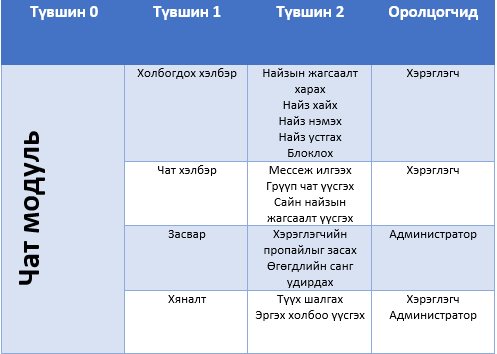
\includegraphics[scale=0.9]{Chart/Chart9}
	\caption[Юзкейс диаграм]{Юзкейс диаграмын хүснэгт}
	\label{fit:UseCase}
\end{figure}
\begin{figure}[htbp]
	\centering
	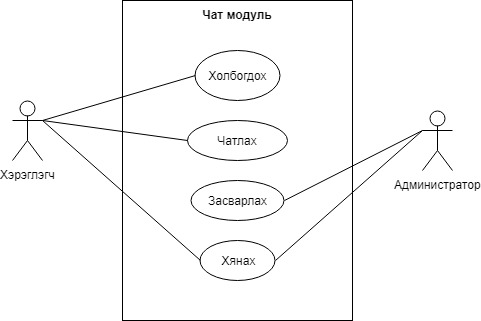
\includegraphics[scale=0.6]{Diagrams/UseCaseMain}
	\caption[Юзкейс диаграм]{Юзкейс диаграм}
	\label{fit:UseCase}
\end{figure}
\begin{figure}[htbp]
	\centering
	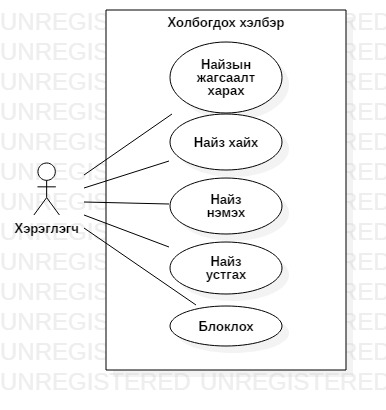
\includegraphics[scale=0.4]{Diagrams/UseCaseContactForm}
	\caption[Юзкейс диаграм]{Юзкейс диаграм (Холбогдох хэлбэр)}
	\label{fit:UseCase}
\end{figure}
\begin{figure}[htbp]
	\centering
	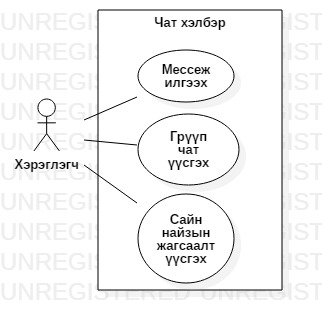
\includegraphics[scale=0.4]{Diagrams/UseCaseChatForm}
	\caption[Юзкейс диаграм]{Юзкейс диаграм (Чат хэлбэр)}
	\label{fit:UseCase}
\end{figure}
\begin{figure}[htbp]
	\centering
	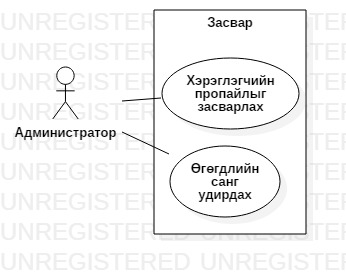
\includegraphics[scale=0.4]{Diagrams/UseCaseMaintenance}
	\caption[Юзкейс диаграм]{Юзкейс диаграм (Засвар)}
	\label{fit:UseCase}
\end{figure}
\begin{figure}[htbp]
	\centering
	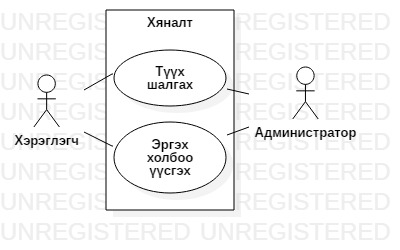
\includegraphics[scale=0.4]{Diagrams/UseCaseMonitor}
	\caption[Юзкейс диаграм]{Юзкейс диаграм (Хяналт)}
	\label{fit:UseCase}
\end{figure}
